\begin{figure}[!ht]
        \subfigure{
        \centering
            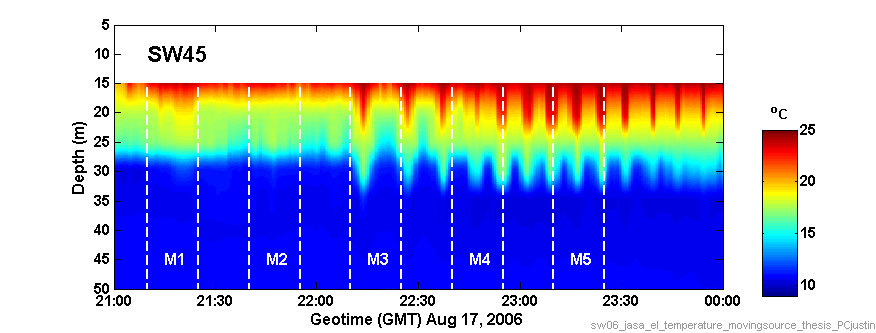
\includegraphics[width=0.8\textwidth]{jasa_el_sw45_movingsource_thesis.png}
            \label{fig:sw45_fix}}
        \subfigure{
            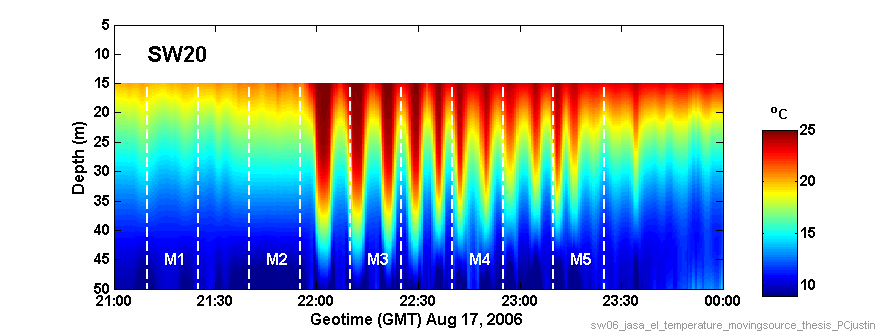
\includegraphics[width=0.8\textwidth]{jasa_el_sw20_movingsource_thesis.png}
            \label{fig:sw20_fix}}
        \subfigure{
            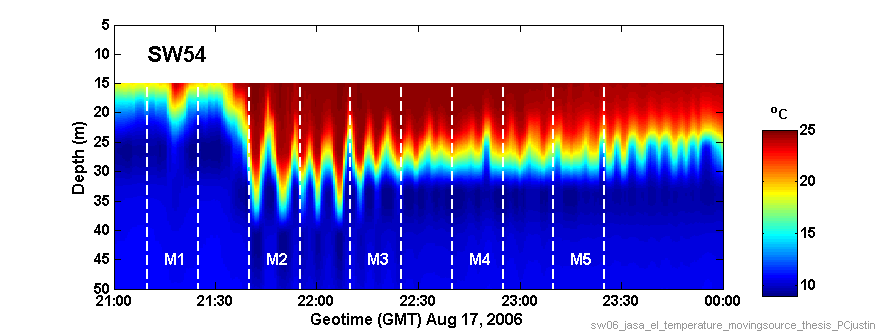
\includegraphics[width=0.8\textwidth]{jasa_el_sw54_movingsource_thesis.png}
            \label{fig:sw54_fix}}
    \caption{Temperature record at three location along the fixed sourc-receiver track. Panel (a), (b) and (c) show the temperature at the NRL300 source (SW45), the midpoint (SW20) and the Shark VLA (SW54).}
    \label{fig:j15_temp}
\end{figure}
%%--M1
\begin{figure}[H]
  \centering
  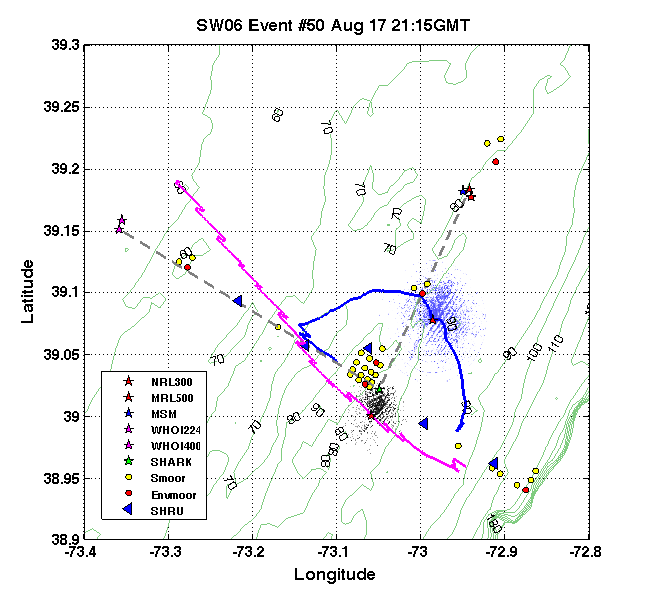
\includegraphics[width=\textwidth]{Aug17_2115_t.png}
  \caption{Surface expression of internal wave package at 21:15GMT, Aug. 17, recorded by R/V Sharp and R/V Oceanus. Blue and red lines indicate their movements, respectively. (Blue: R/V Sharp's, red: R/V Oceanus'}\label{fig:r2115_r}
\end{figure}

%\begin{figure}[H]
% \centering
% 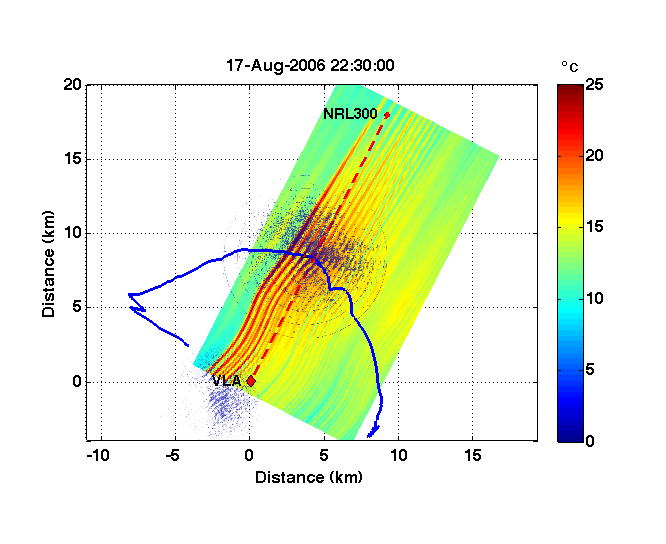
\includegraphics[width=\textwidth]{sw06_Tempr_Depth30m_2006Aug17_223000_radar_curve_thesis1.png}
% \caption{Interpolated internal wave field at 22:30GMT, Aug. 17, water depth = 20m. (Refer to section 3.4 for detailed interpolation method)}\label{fig:r2130_i}
%\end{figure}

\begin{figure}[H]
  \centering
  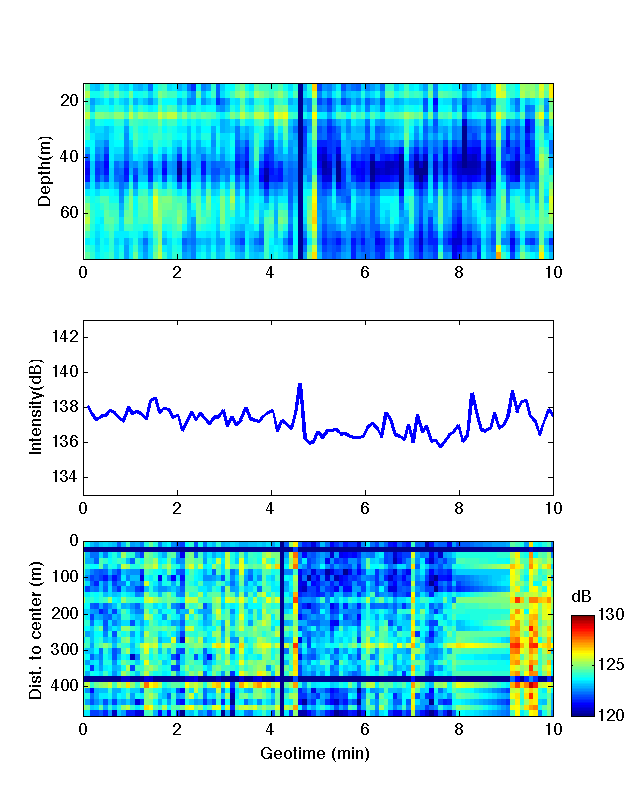
\includegraphics[width=\textwidth]{udel_060817T2115_vla_hla_intens_geotime2.png}
  \caption{Received signal on Shark VLA (top), HLA (bottom) and signal intensity (middle) from Aug.17 21:15GMT to 21:25GMT }\label{fig:a2115}
\end{figure}

%\begin{figure}[h]
%\centering
% 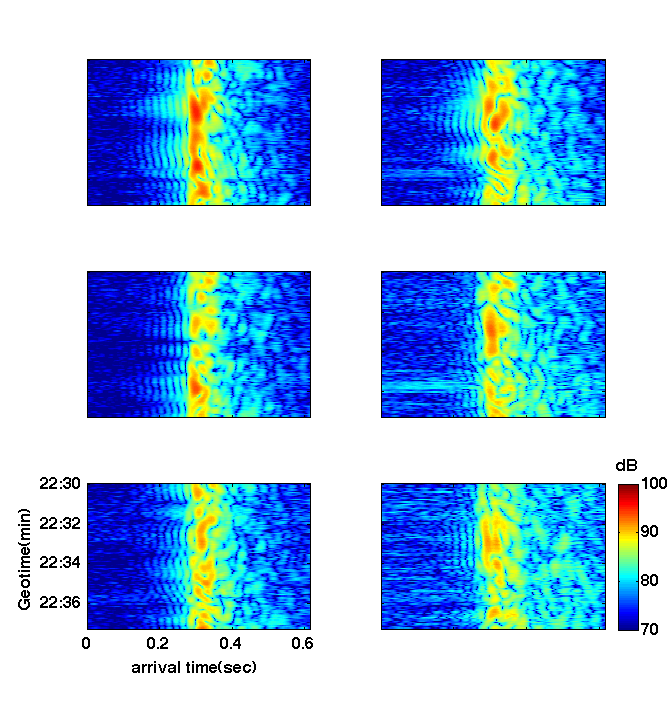
\includegraphics[width=\textwidth]{sw06_broadband_mf_nrl300_F5_6in1_thesis.png}
%  \caption{Mode decomposition of received signal on Shark VLA. 
 %   Left column: mode 1-3, right column: mode 4-6 }\label{fig:m2130}
%\end{figure}


%%--M2
\begin{figure}[H]
  \centering
  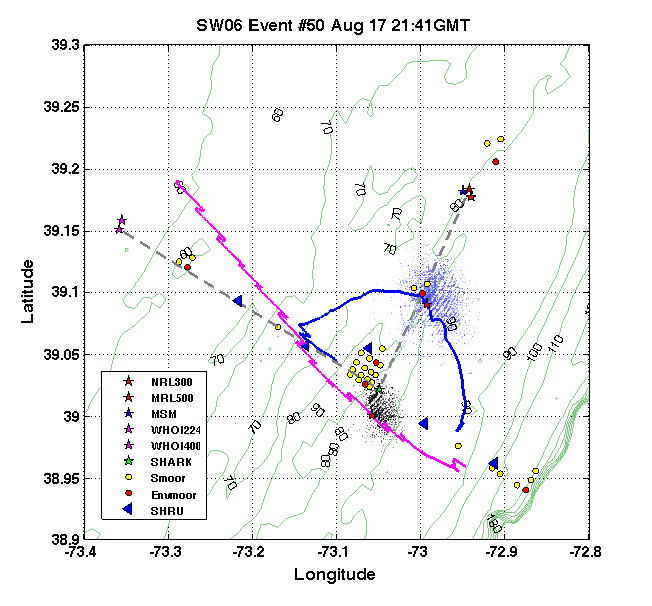
\includegraphics[width=\textwidth]{Aug17_2141_t.png}
  \caption{Surface expression of internal wave package at 21:41GMT, Aug. 17, recorded by R/V Sharp and R/V Oceanus. Blue and red lines indicate their movements, respectively. (Blue: R/V Sharp's, red: R/V Oceanus'}\label{fig:r2141_r}
\end{figure}

%\begin{figure}[H]
% \centering
% 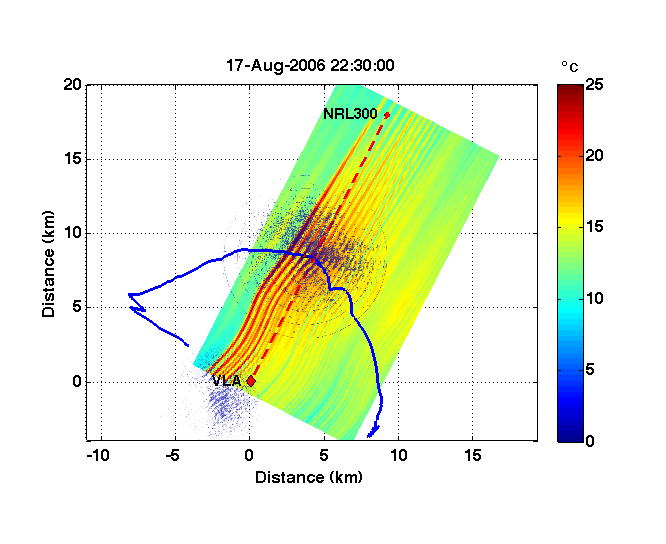
\includegraphics[width=\textwidth]{sw06_Tempr_Depth30m_2006Aug17_223000_radar_curve_thesis1.png}
% \caption{Interpolated internal wave field at 22:30GMT, Aug. 17, water depth = 20m. (Refer to section 3.4 for detailed interpolation method)}\label{fig:r2130_i}
%\end{figure}

\begin{figure}[H]
  \centering
  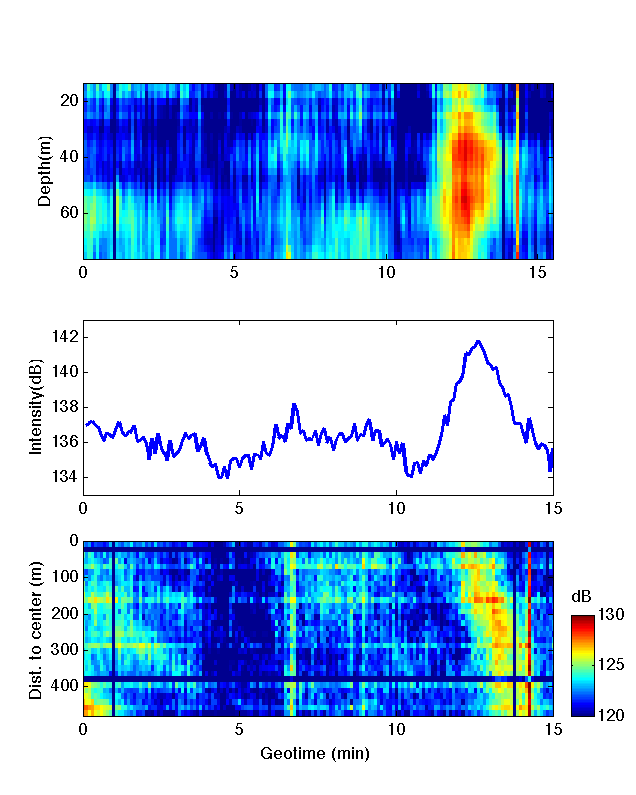
\includegraphics[width=\textwidth]{udel_060817T2141_vla_hla_intens_geotime2.png}
  \caption{Received signal on Shark VLA (top), HLA (bottom) and signal intensity (middle) from Aug.17 21:41GMT to 21:56GMT }\label{fig:a2141}
\end{figure}

%\begin{figure}[h]
%\centering
% 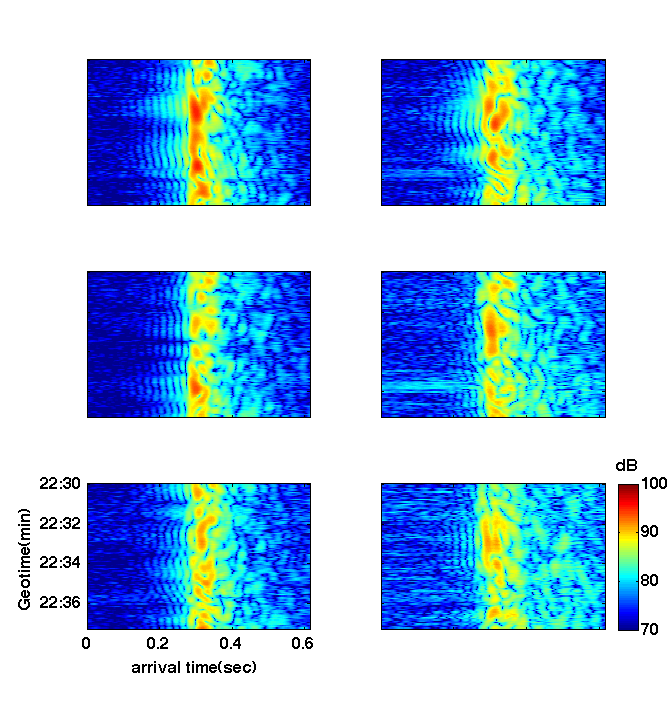
\includegraphics[width=\textwidth]{sw06_broadband_mf_nrl300_F5_6in1_thesis.png}
%  \caption{Mode decomposition of received signal on Shark VLA. 
 %   Left column: mode 1-3, right column: mode 4-6 }\label{fig:m2130}
%\end{figure}


%%--M3
\begin{figure}[H]
  \centering
  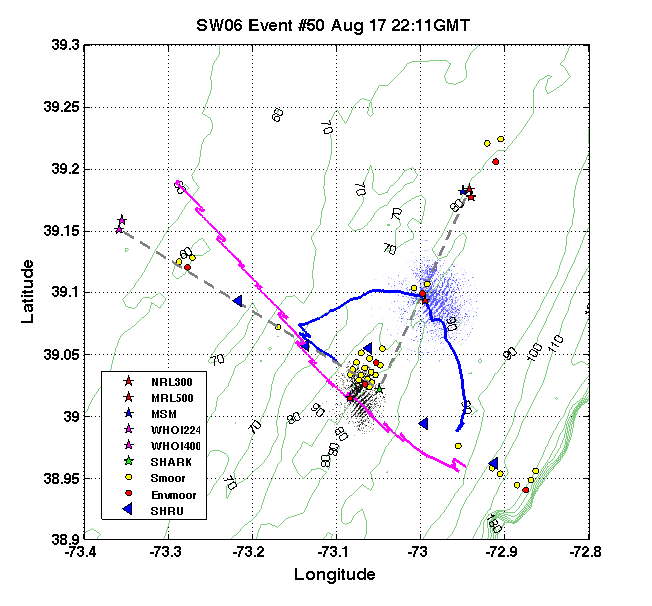
\includegraphics[width=\textwidth]{Aug17_2211_t.png}
  \caption{Surface expression of internal wave package at 22:11GMT, Aug. 17, recorded by R/V Sharp and R/V Oceanus. Blue and red lines indicate their movements, respectively. (Blue: R/V Sharp's, red: R/V Oceanus'}\label{fig:r2211_r}
\end{figure}

%\begin{figure}[H]
% \centering
% 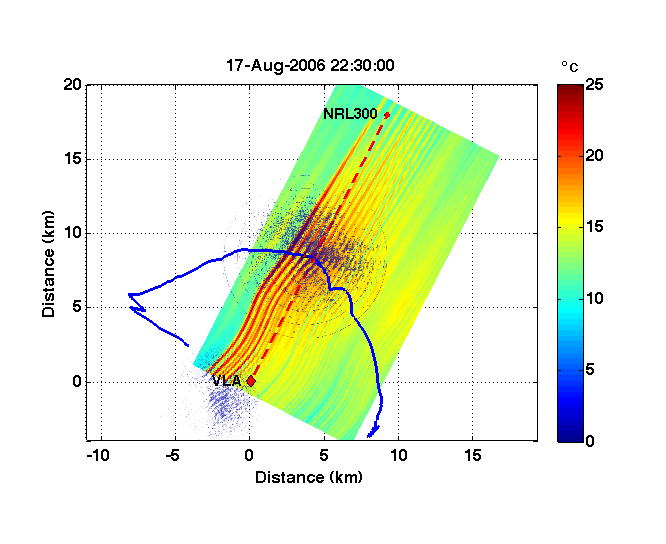
\includegraphics[width=\textwidth]{sw06_Tempr_Depth30m_2006Aug17_223000_radar_curve_thesis1.png}
% \caption{Interpolated internal wave field at 22:30GMT, Aug. 17, water depth = 20m. (Refer to section 3.4 for detailed interpolation method)}\label{fig:r2130_i}
%\end{figure}

\begin{figure}[H]
  \centering
  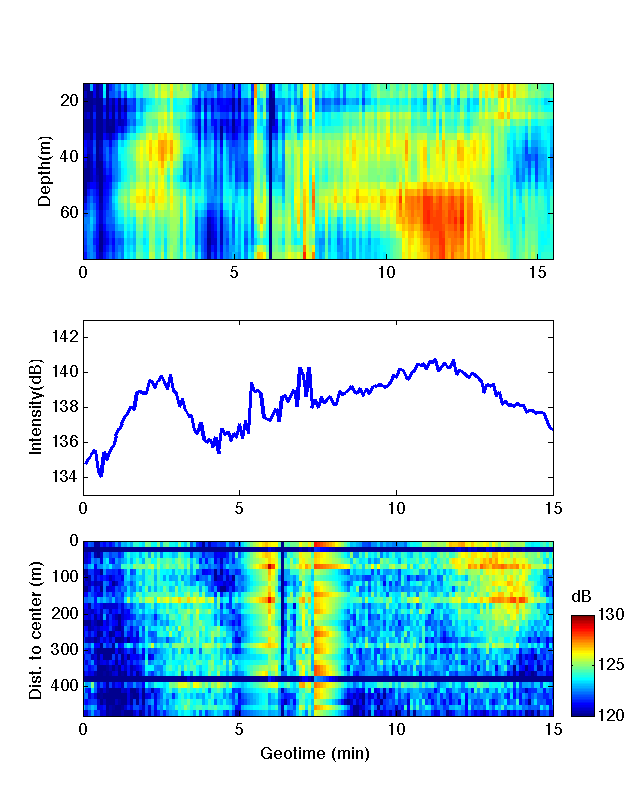
\includegraphics[width=\textwidth]{udel_060817T2211_vla_hla_intens_geotime2.png}
  \caption{Received signal on Shark VLA (top), HLA (bottom) and signal intensity (middle) from Aug.17 22:11GMT to 22:26GMT }\label{fig:a2211}
\end{figure}

%\begin{figure}[h]
%\centering
% 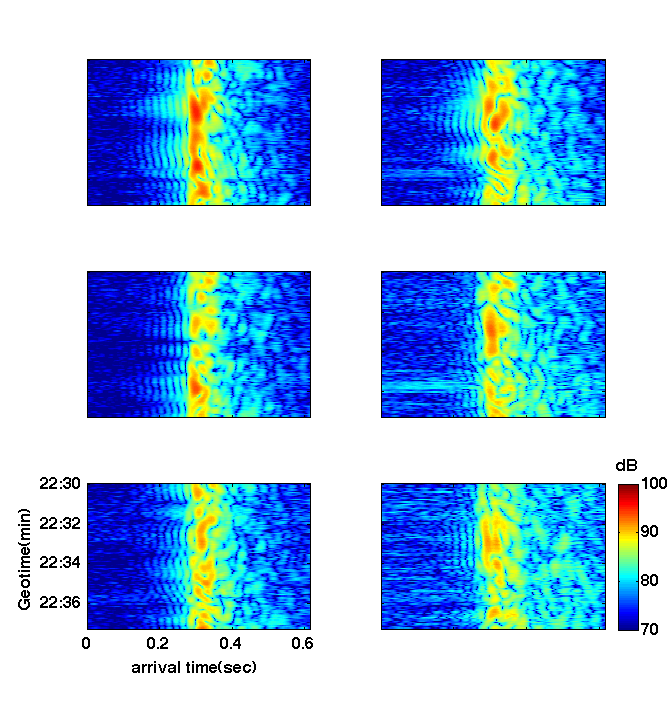
\includegraphics[width=\textwidth]{sw06_broadband_mf_nrl300_F5_6in1_thesis.png}
%  \caption{Mode decomposition of received signal on Shark VLA. 
 %   Left column: mode 1-3, right column: mode 4-6 }\label{fig:m2130}
%\end{figure}


%%--M4
\begin{figure}[H]
  \centering
  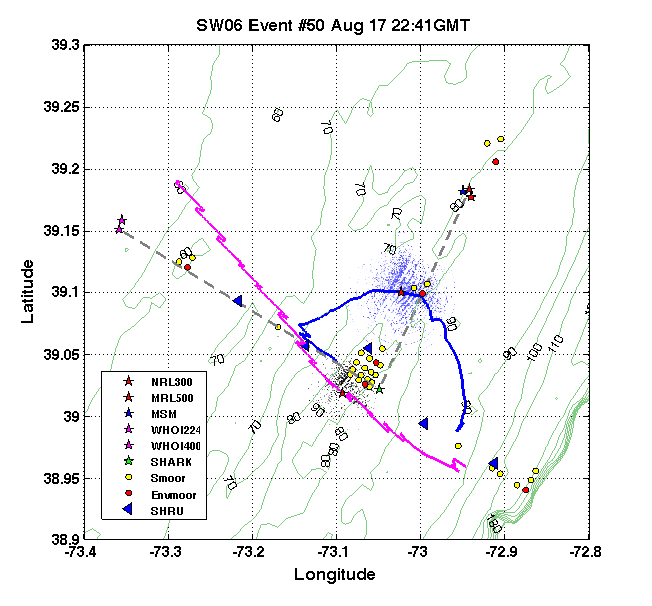
\includegraphics[width=\textwidth]{Aug17_2241_t.png}
  \caption{Surface expression of internal wave package at 22:41GMT, Aug. 17, recorded by R/V Sharp and R/V Oceanus. Blue and red lines indicate their movements, respectively. (Blue: R/V Sharp's, red: R/V Oceanus'}\label{fig:r2241_r}
\end{figure}

%\begin{figure}[H]
% \centering
% 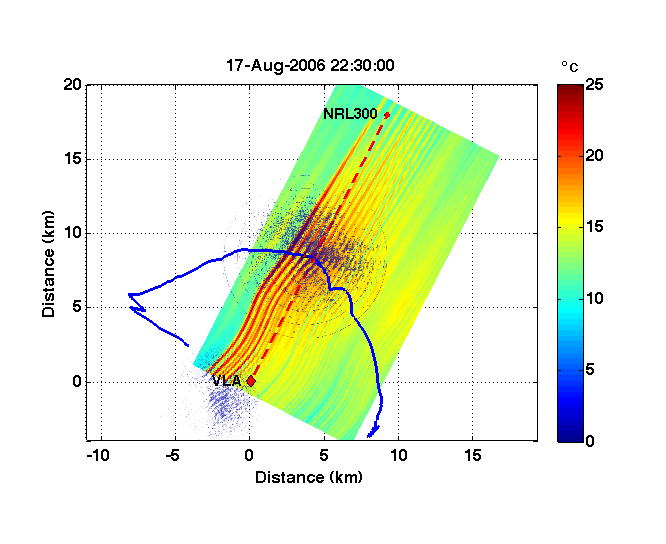
\includegraphics[width=\textwidth]{sw06_Tempr_Depth30m_2006Aug17_223000_radar_curve_thesis1.png}
% \caption{Interpolated internal wave field at 22:30GMT, Aug. 17, water depth = 20m. (Refer to section 3.4 for detailed interpolation method)}\label{fig:r2130_i}
%\end{figure}

\begin{figure}[H]
  \centering
  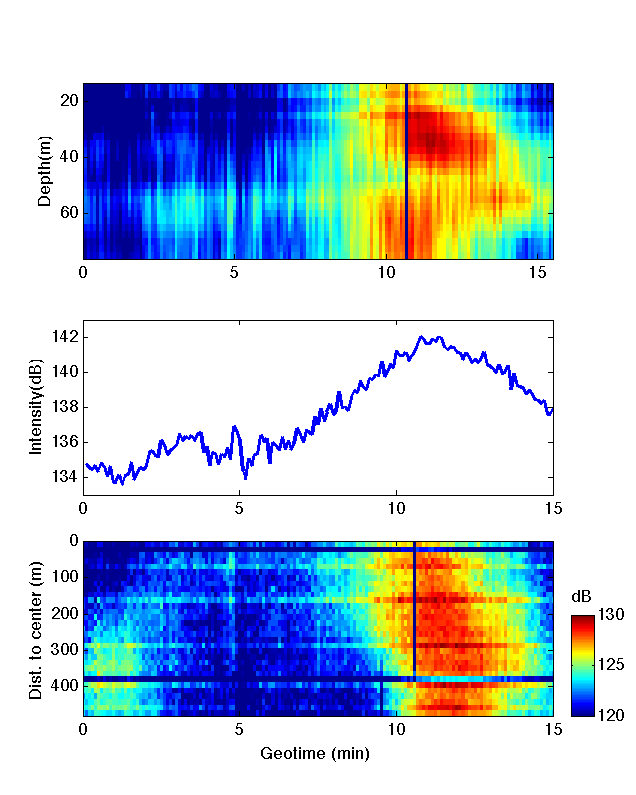
\includegraphics[width=\textwidth]{udel_060817T2241_vla_hla_intens_geotime2.png}
  \caption{Received signal on Shark VLA (top), HLA (bottom) and signal intensity (middle) from Aug.17 22:41GMT to 22:46GMT }\label{fig:a2241}
\end{figure}

%\begin{figure}[h]
%\centering
% 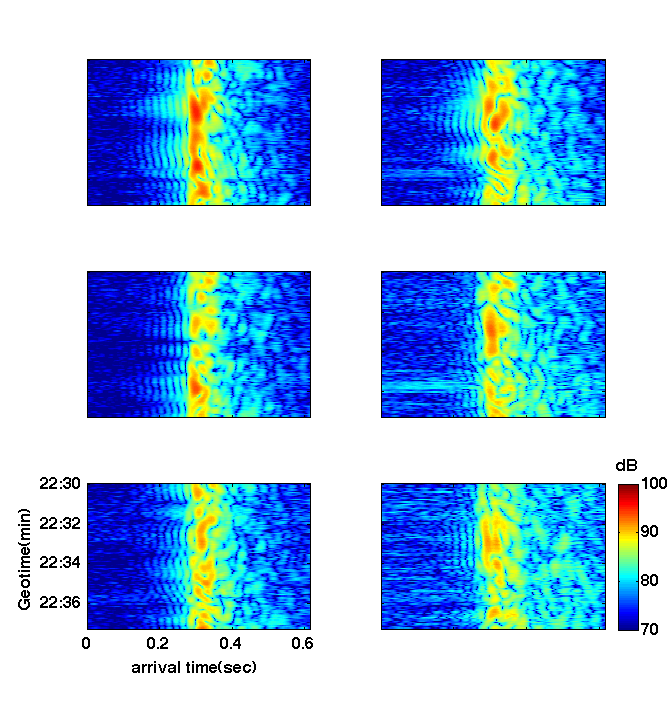
\includegraphics[width=\textwidth]{sw06_broadband_mf_nrl300_F5_6in1_thesis.png}
%  \caption{Mode decomposition of received signal on Shark VLA. 
 %   Left column: mode 1-3, right column: mode 4-6 }\label{fig:m2130}
%\end{figure}


%%--M5
\begin{figure}[H]
  \centering
  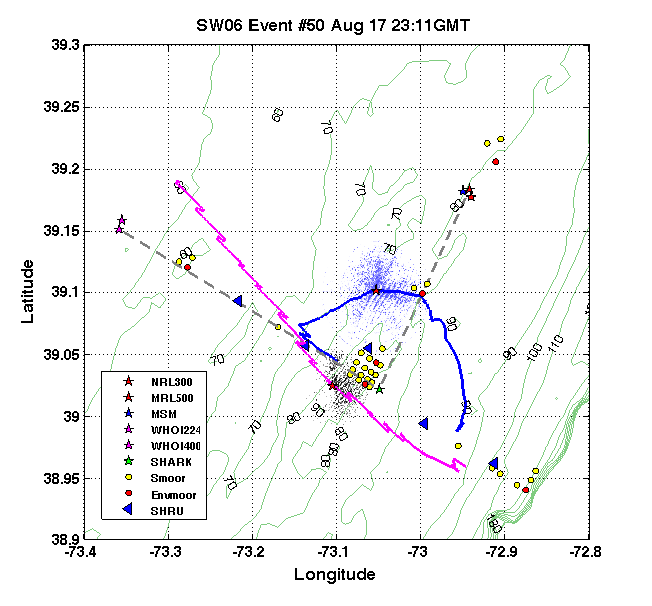
\includegraphics[width=\textwidth]{Aug17_2311_t.png}
  \caption{Surface expression of internal wave package at 23:11GMT, Aug. 17, recorded by R/V Sharp and R/V Oceanus. Blue and red lines indicate their movements, respectively. (Blue: R/V Sharp's, red: R/V Oceanus'}\label{fig:r2311_r}
\end{figure}

%\begin{figure}[H]
% \centering
% 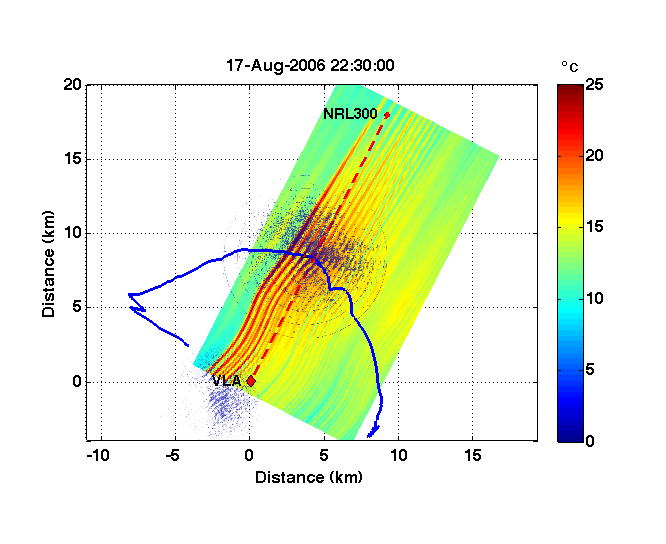
\includegraphics[width=\textwidth]{sw06_Tempr_Depth30m_2006Aug17_223000_radar_curve_thesis1.png}
% \caption{Interpolated internal wave field at 22:30GMT, Aug. 17, water depth = 20m. (Refer to section 3.4 for detailed interpolation method)}\label{fig:r2130_i}
%\end{figure}

\begin{figure}[H]
  \centering
  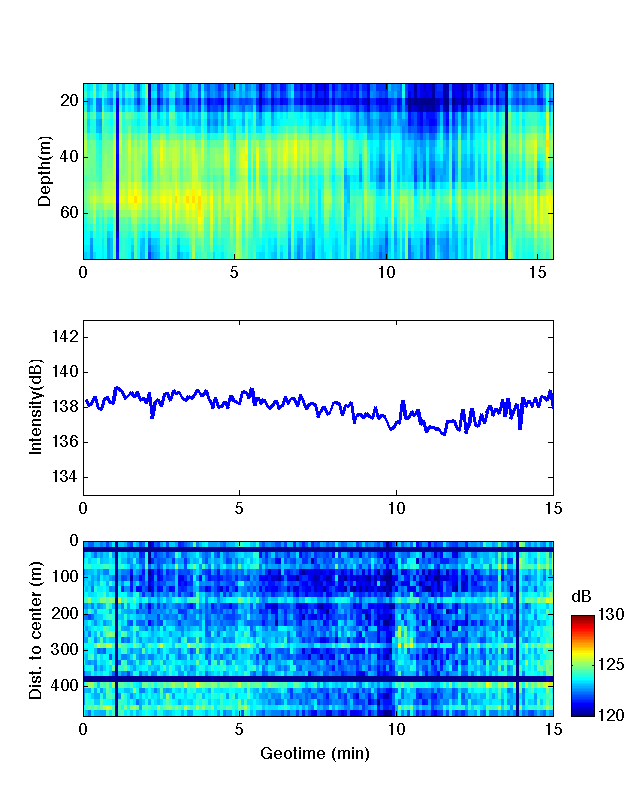
\includegraphics[width=\textwidth]{udel_060817T2311_vla_hla_intens_geotime2.png}
  \caption{Received signal on Shark VLA (top), HLA (bottom) and signal intensity (middle) from Aug.17 23:11GMT to 23:26GMT }\label{fig:a2311}
\end{figure}



\clearpage


\begin{figure}[H]
  \centering
  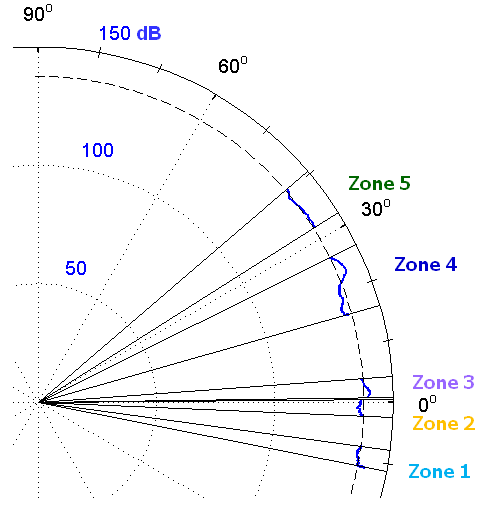
\includegraphics[width=0.6\textwidth]{angular_distr_4.png}
  \caption{Data of depth-integrated intensity and estimated angle for each zone }\label{fig:a2130}
\end{figure}

